\chapter{Sequence modeling}


\section{Memoryless approach}
\marginnote{Memoryless approach}

Neural network that takes as input a fixed number of elements of the sequence.

\begin{remark}
    They are not ideal for long-term dependencies.
\end{remark}



\section{Recurrent neural network}

\begin{description}
    \item[Recurrent neural network (RNN)] \marginnote{Recurrent neural network}
        Neural network in which hidden states have backward connections in such a way that each state depends on the past history.

        Inputs are processed one time step at a time as they cannot be parallelized since each step needs the hidden state at the previous time step.

        \begin{figure}[H]
            \centering
            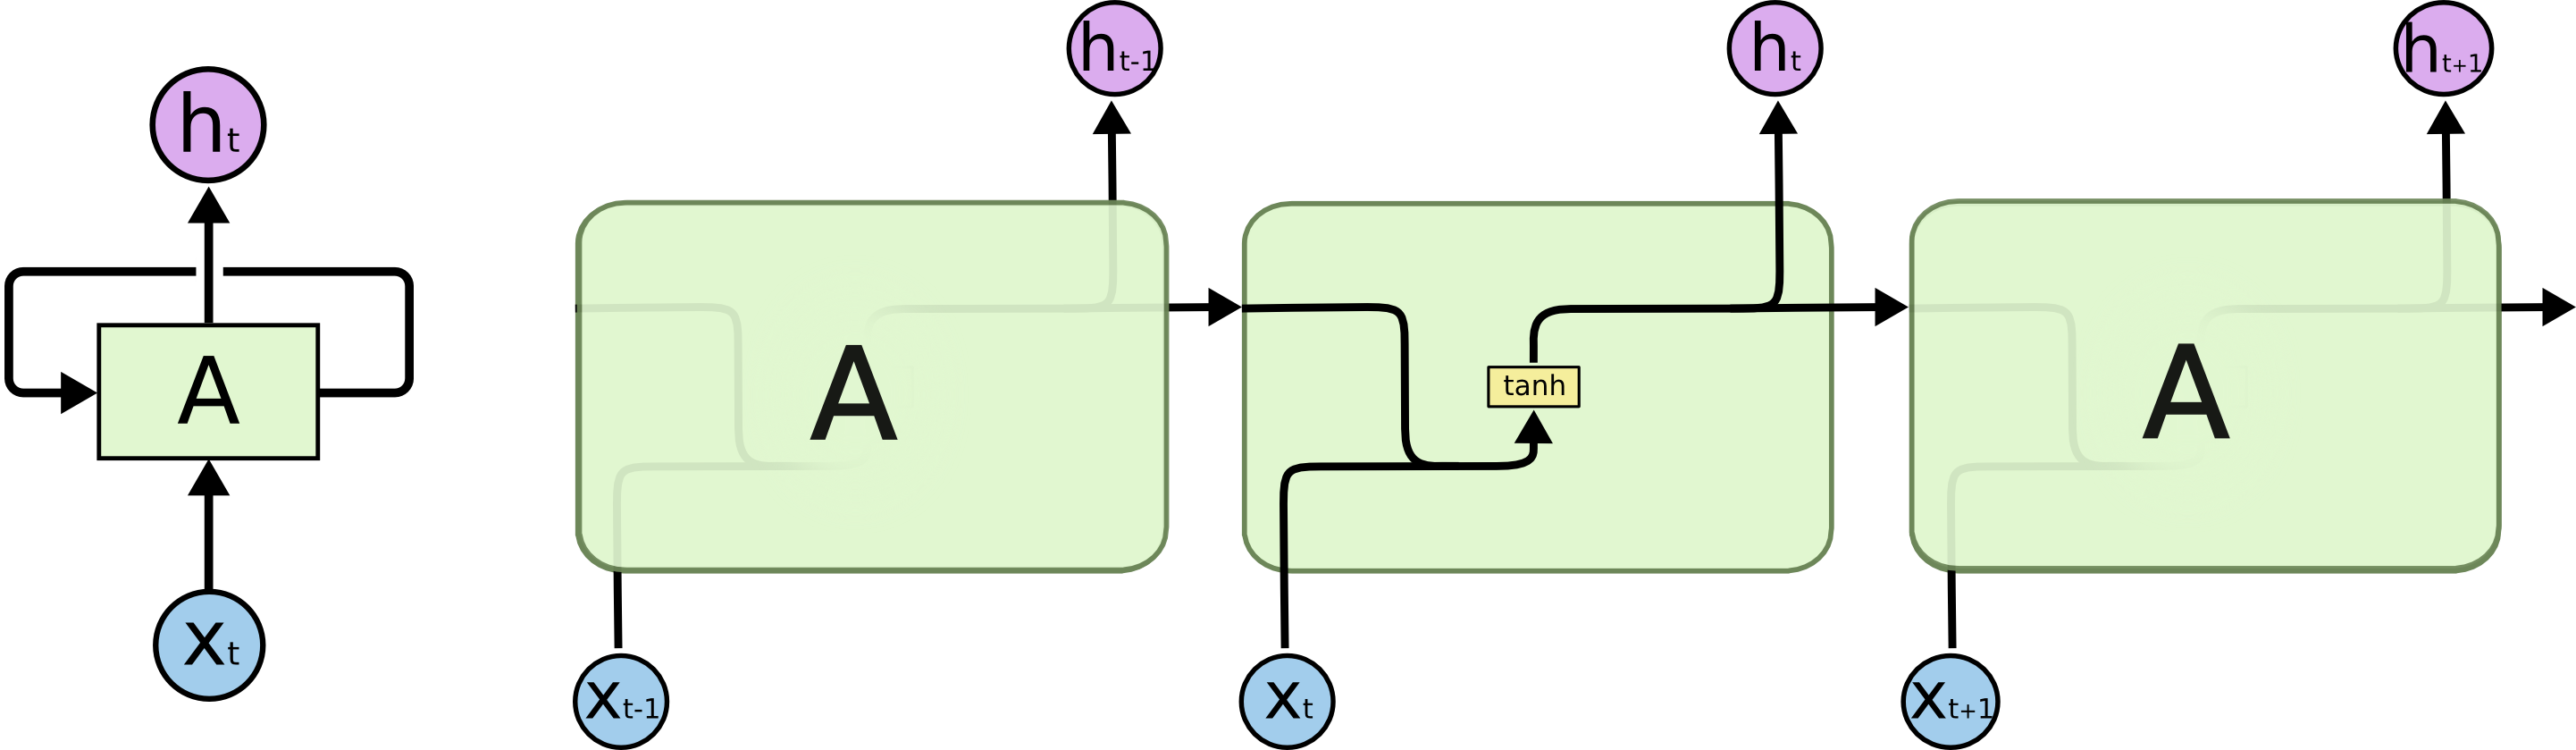
\includegraphics[width=0.65\linewidth]{./img/rnn.png}
            \caption{Example of RNN (left) and its unfolded version (right)}
        \end{figure}

    \item[Backpropagation] \marginnote{RNN backpropagation}
        Weight updates in RNNs are computed by averaging the gradients of each time step (i.e. a forward pass involves processing an entire sequence).

        By seeing an RNN in its unfolded form, this way of updating the weights guarantees that the parameters of the network remain the same for each time step.

        \begin{remark}
            For long sequences, it is very easy for the gradient to explode or vanish.
        \end{remark}

    \item[Hidden state initialization] \marginnote{Hidden state initialization}
        There are different ways to set the initial hidden state at $t=0$:
        \begin{itemize}
            \item Initialize to zero.
            \item Sample from a known distribution.
            \item Learned during training.
        \end{itemize}
\end{description}



\subsection{Long-short term memory}
\marginnote{Long-short term memory}

Traditional RNNs usually only carry to the next time step the output of the current step.

Long-short term memory is an architecture of RNN that, along side the output of the previous layer, allows the model itself to learn what to "remember".

\begin{figure}[H]
    \centering
    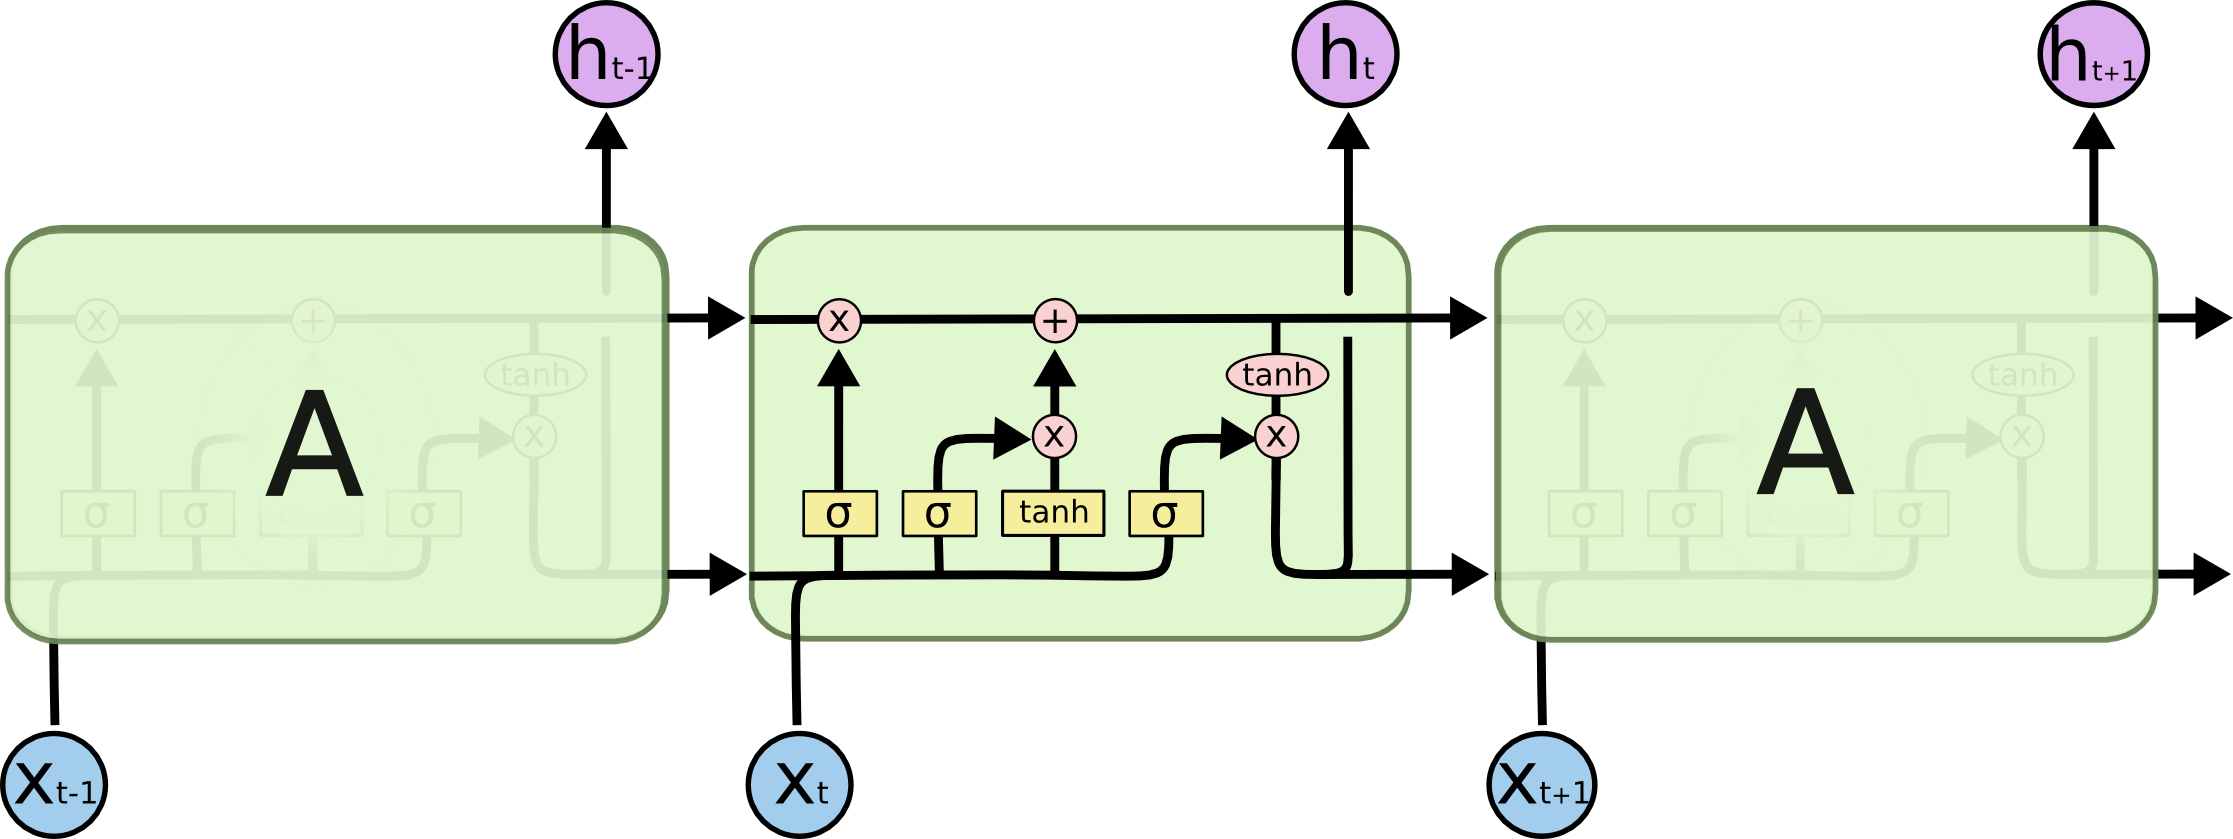
\includegraphics[width=0.6\linewidth]{./img/lstm.png}
\end{figure}


Let:
\begin{itemize}
    \item $W_g$ and $b_g$ be the weights and biases of the component $g$,
    \item $h_t$ the output of at time step $t$,
    \item $x_t$ the input at time step $t$,
\end{itemize}
an LSTM has the following components:
\begin{descriptionlist}
    \item[Forget gate] 
        Computes a mask $f_t$ that will decide which part of the memory to preserve.\\
        \begin{minipage}{0.6\linewidth}
            \[ f_t = \sigma( W_f \cdot [h_{t-1}, x_t] + b_f) \]
        \end{minipage}
        \begin{minipage}{0.35\linewidth}
            \centering
            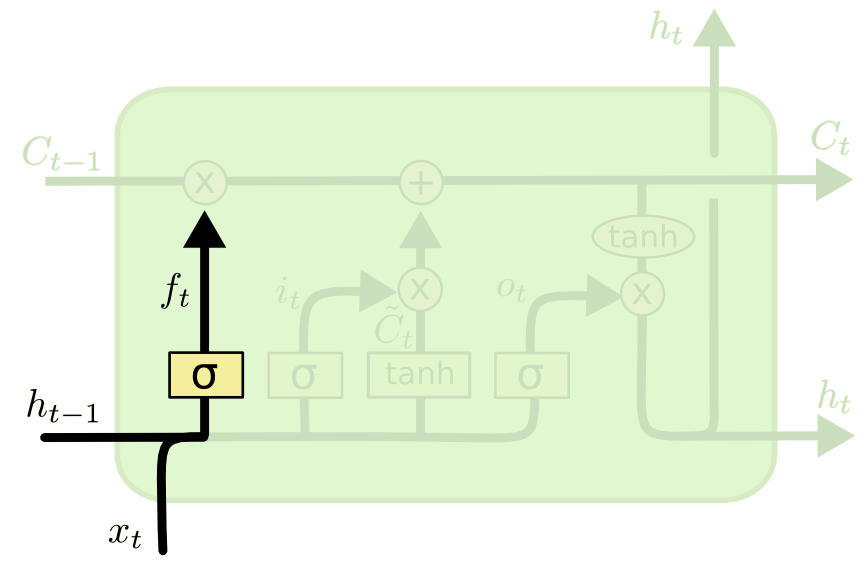
\includegraphics[width=0.85\linewidth]{./img/forget_gate.png}
        \end{minipage}

    \item[Update gate] 
        It is composed of two parts:
        \begin{descriptionlist}
            \item[Input gate] Computes a mask $i_t$ that decides which part of the input to preserve.
            \item[\texttt{tanh} layer] Creates a vector $\tilde{C}_t$ of new candidate values to potentially be saved in the memory.
        \end{descriptionlist}
        \begin{minipage}{0.6\linewidth}
            \[
                \begin{split}
                    i_t &= \sigma( W_i \cdot [h_{t-1}, x_t] + b_i) \\
                    \tilde{C}_t &= \texttt{tanh}( W_C \cdot [h_{t-1}, x_t] + b_C) \\
                \end{split}
            \]
        \end{minipage}
        \begin{minipage}{0.35\linewidth}
            \centering
            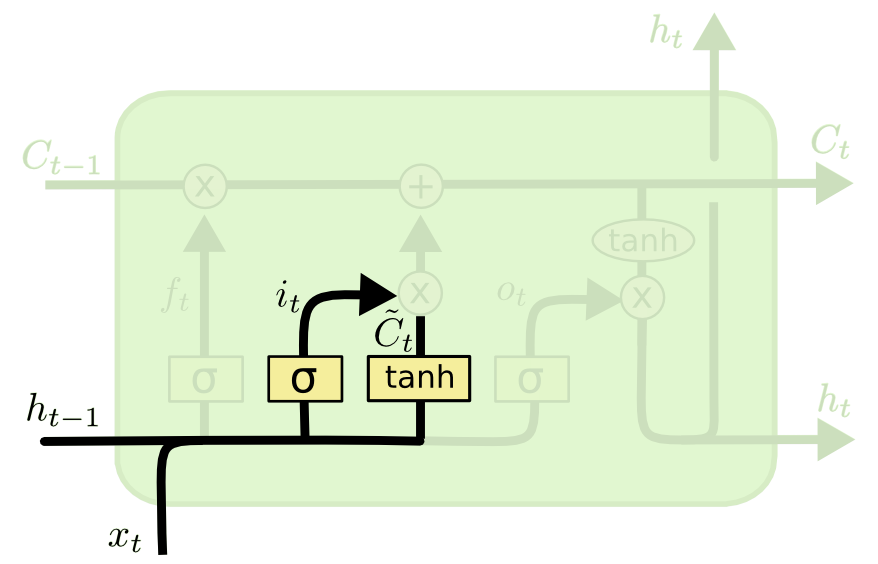
\includegraphics[width=0.85\linewidth]{./img/update_gate.png}
        \end{minipage}

    \item[C-line] 
        Represents the memory of the network.
        At each step, the memory $C_{t-1}$ of the previous step is updated and a new state $C_t$ is outputted to the next step.\\
        \begin{minipage}{0.6\linewidth}
            \[ C_t = f_t * C_{t-1} + i_t * \tilde{C}_t \]
        \end{minipage}
        \begin{minipage}{0.35\linewidth}
            \centering
            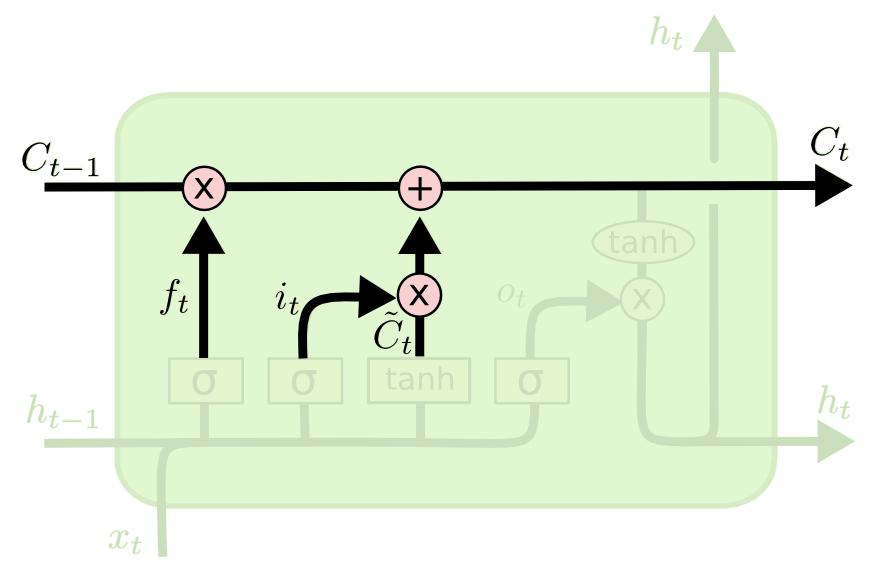
\includegraphics[width=0.85\linewidth]{./img/cline_update.png}
        \end{minipage}

    \item[Output gate] 
        The output $h_t$ at step $t$ is determined by the current input and the updated memory.\\
        \begin{minipage}{0.6\linewidth}
            \[
                \begin{split}
                    o_t &= \sigma( W_o \cdot [h_{t-1}, x_t] + b_o) \\
                    h_t &= o_t * \texttt{tanh}(C_t) \\
                \end{split}
            \]
        \end{minipage}
        \begin{minipage}{0.35\linewidth}
            \centering
            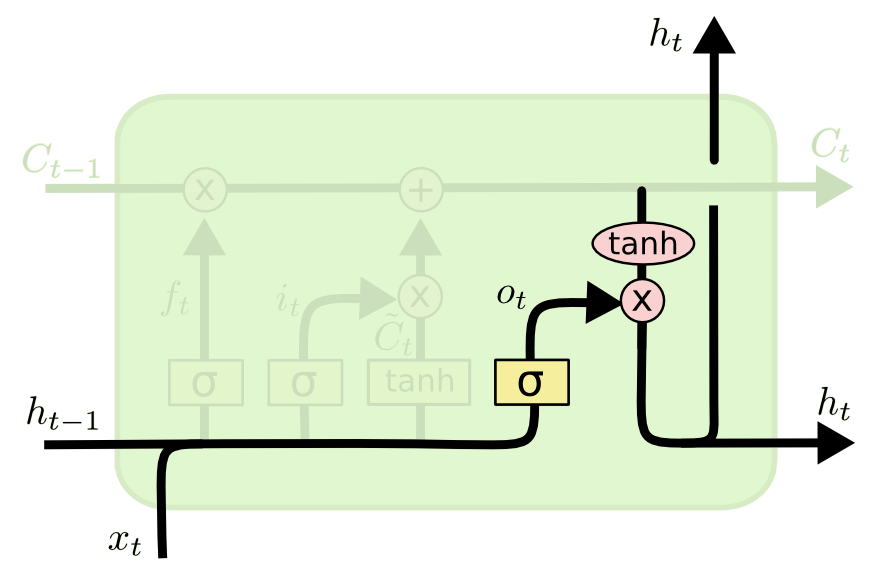
\includegraphics[width=0.85\linewidth]{./img/output_gate.png}
        \end{minipage}
\end{descriptionlist}